\documentclass[10pt,aspectratio=169]{beamer}
\usepackage[utf8]{inputenc}
\usepackage[T1]{fontenc}
\usepackage{lmodern}
\usepackage{amsmath}
\usepackage{amsfonts}
\usepackage{amssymb}
\usepackage{graphicx}
\usepackage{hyperref}
\usepackage{listings}
\usepackage{xcolor}
\usepackage{soul}
\usepackage[11pt]{moresize}
\usepackage{multirow}

\definecolor{codegreen}{rgb}{0,0.6,0}
\definecolor{codegray}{rgb}{0.5,0.5,0.5}
\definecolor{codepurple}{rgb}{0.58,0,0.82}
\definecolor{backcolour}{rgb}{0.95,0.95,0.92}

\lstdefinestyle{standard}{
	backgroundcolor=\color{backcolour},   
	commentstyle=\color{codegreen},
	keywordstyle=\color{magenta},
	numberstyle=\color{codegray},
	stringstyle=\color{codepurple},
	basicstyle=\ttfamily\scriptsize,
	breakatwhitespace=false,         
	breaklines=true,                 
	captionpos=b,                    
	keepspaces=true,                 
	showspaces=false,                
	showstringspaces=false,
	showtabs=false,                  
	framesep=0mm,
	tabsize=4
}
\lstset{style=standard}
\lstset{escapeinside={(*@}{@*)}}

\AtBeginSection[]{
	\begin{frame}
		\vfill
		\centering
		\begin{beamercolorbox}[sep=8pt,center,shadow=true,rounded=true]{title}
			\usebeamerfont{title}\insertsectionhead\par%
		\end{beamercolorbox}
		\vfill
	\end{frame}
}

\usetheme{Singapore}
\begin{document}
	\author{Quan Gan}
	\title{Introduction to DGL}
	%\subtitle{}
	%\logo{}
	\institute{AWS Shanghai AI Lab}
	%\date{}
	%\subject{}
	%\setbeamercovered{transparent}
	\setbeamertemplate{navigation symbols}{}
	\begin{frame}[plain]
		\maketitle
	\end{frame}

	\begin{frame}
		\frametitle{What does DGL provide?}
		\begin{itemize}
			\item From bottom-level to top-level:
			\begin{itemize}
				\item \emph{Plug-and-play model zoo}, to run an existing model on your data directly
				\item \emph{Easy-to-use graph neural network layer modules}, to plugin popular GNN layers into your model.
				\item \emph{Flexible and efficient message passing APIs}, to design your own message passing (not necessarily full-graph!) from scratch.
			\end{itemize}
		\end{itemize}
	\end{frame}
	
	\begin{frame}[fragile]
		\frametitle{Model Zoo?}
		\begin{itemize}
			\item Get a (pretrained) model that works on molecules immediately:
\begin{lstlisting}[language=Python]
from dgl.model_zoo.chem import load_pretrained
model = load_pretrained('MPNN_Alchemy')
result = model(molecule, atom_features, bond_features)
\end{lstlisting}
			\item We just released a subpackage \emph{DGL-KE} for training embeddings on large scale knowledge graphs such as FreeBase.
			\item We are shooting for a model zoo for recommender systems in 0.5.
		\end{itemize}
	\end{frame}

	\begin{frame}[fragile]
		\frametitle{Graph Neural Network Layer Modules?}
		\begin{itemize}
			\item Use DGL GNN Modules to build a bigger network:
\begin{lstlisting}[language=Python]
from dgl.nn.pytorch import SAGEConv

# One layer GraphSAGE
class NodeClassifier(nn.Module):
    def __init__(self, in_dim, n_classes):
        self.gnn = SAGEConv(in_dim, in_dim, 'mean')
        self.cls = nn.Linear(in_dim, n_classes)
    def forward(self, g, x):
        h = self.gnn(g, x)
        return self.cls(h)
\end{lstlisting}
			\item We have lots of popular GNN modules implemented.
			\begin{itemize}
				\item The list is growing!
			\end{itemize}
		\end{itemize}
	\end{frame}
	
	\begin{frame}
		\frametitle{Custom Graph Neural Network Layer?}
		$$
		h^{(k)}_v = \phi\left(
		h^{(k-1)}_v,
		h^{(k)}_{\mathcal{N}(v)}
		\right) \qquad h^{(k)}_{\mathcal{N}(v)} = f\left(
		\left\lbrace
		h^{(k-1)}_u : u \in \mathcal{N}(v)
		\right\rbrace
		\right) \footnote{Xu et al., \emph{How Powerful Are Graph Neural Networks?}, ICLR 2019}
		$$
		\begin{center}
			\centering
			\only<1>{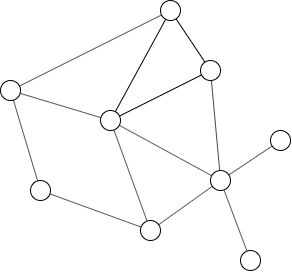
\includegraphics[width=0.4\textwidth]{graph-1.png}}
			\only<2>{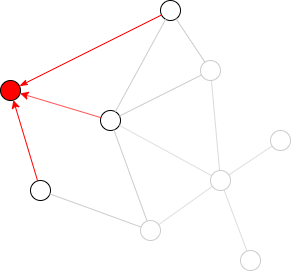
\includegraphics[width=0.4\textwidth]{graph-2.png}}
			\only<3>{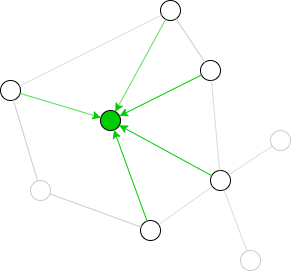
\includegraphics[width=0.4\textwidth]{graph-3.png}}
			\only<4>{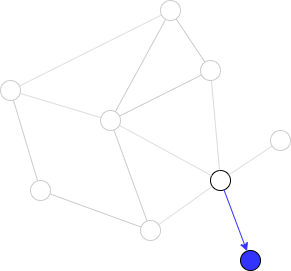
\includegraphics[width=0.4\textwidth]{graph-4.png}}
		\end{center}
	\end{frame}

	\begin{frame}[fragile]
		\frametitle{Aggregation: Average Pooling\footnote{Hamilton et al., \emph{Inductive Representation Learning on Large Graphs}, NIPS 2017}}
		\begin{minipage}{0.5\textwidth}
			Sparse matrix multiplication, very well-known:
\begin{lstlisting}[language=Python]
# code: PyTorch
# src: edge source node IDs (n_nodes,)
# dst: edge destination node IDs (n_nodes,)
# H: node repr matrix (n_nodes, in_dim)
# W: weights (in_dim * 2, out_dim)
A = torch.sparse_coo_tensor(
    torch.stack([dst, src], 0),
    torch.ones(n_nodes),
    (n_nodes, n_nodes))
in_deg = torch.sparse.sum(A, 1).to_dense()
H_N = A @ H / in_deg.unsqueeze(1)
H = torch.relu(torch.cat([H_N, H], 1) @ W)
\end{lstlisting}
		\end{minipage}%
		\begin{minipage}{0.5\textwidth}
\begin{lstlisting}[language=Python]
# code: PyTorch + DGL
# G: DGL Graph
# H: node repr matrix (n_nodes, in_dim)
# W: weights (in_dim * 2, out_dim)
import dgl.function as fn
G.ndata['h'] = H
G.update_all(
    fn.copy_u('h', 'm'),
    fn.mean('m', 'h_n'))
H_N = G.ndata['h_n']
H = torch.relu(torch.cat([H_N, H], 1) @ W)
\end{lstlisting}
		\end{minipage}
	\end{frame}

	\begin{frame}[fragile]
		\frametitle{How about max pooling?}
		
			Not possible in Vanilla PyTorch \& MXNet.  Not memory-efficient in Tensorflow.
\begin{minipage}{0.5\textwidth}
\begin{lstlisting}[language=Python]
# code: Tensorflow 2
# src: edge source node IDs (n_nodes,)
# dst: edge destination node IDs (n_nodes,)
# H: node repr matrix (n_nodes, in_dim)
# W: weights (in_dim * 2, out_dim)

# Broadcast source features to edges
H_src = tf.gather(H, src)
H_N = tf.math.unsorted_segment_max(
    H_src, dst, n_nodes)
H = tf.nn.relu(tf.concat([H_N, H], 1) @ W)
\end{lstlisting}
\end{minipage}%
\begin{minipage}{0.5\textwidth}
\begin{lstlisting}[language=Python]
# code: PyTorch + DGL
# G: DGL Graph
# H: node repr matrix (n_nodes, in_dim)
# W: weights (in_dim * 2, out_dim)
import dgl.function as fn
G.ndata['h'] = H
G.update_all(
    fn.copy_u('h', 'm'),
    fn.(*@\textit{\textcolor{red}{max}}@*)('m', 'h_n'))
H_N = G.ndata['h_n']
H = torch.relu(torch.cat([H_N, H], 1) @ W)
\end{lstlisting}
\end{minipage}
	\end{frame}

	\begin{frame}[fragile]
		\frametitle{With attention?\footnote{Velickovic et al., \emph{Graph Attention Networks}, ICLR 2018}}
		Can't do it easily with vanilla PyTorch/MXNet.  Possible in Tensorflow
		\begin{minipage}{0.5\textwidth}
\begin{lstlisting}[language=Python]
# code: Tensorflow 2
# src: edge source node IDs (n_nodes,)
# dst: edge destination node IDs (n_nodes,)
# H: node repr matrix (n_nodes, in_dim)
# W: weights (in_dim * 2, out_dim)
# SIMPLIFIED - only one attention head is considered
H_src = tf.gather(H, src)
H_dst = tf.gather(H, dst)
alpha_hat = MLP(tf.concat([H_dst, H_src], 1))
alpha_hat_sp = tf.sparse.SparseTensor(
    tf.stack([dst, src], 1),
    alpha_hat,
    (n_nodes, n_nodes))
alpha = tf.sparse.softmax(alpha_hat_sp)
H_N = tf.sparse.sparse_dense_matmul(
    alpha, H)
H = tf.nn.relu(tf.concat([H_N, H], 1) @ W)
\end{lstlisting}
		\end{minipage}%
		\begin{minipage}{0.5\textwidth}
\begin{lstlisting}[language=Python]
# code: PyTorch + DGL
# G: DGL Graph
# H: node repr matrix (n_nodes, in_dim)
# W: weights (in_dim * 2, out_dim)

import dgl.function as fn
G.ndata['h'] = H
G.update_all((*@\textit{\textcolor{red}{msg\_func}}@*), (*@\textit{\textcolor{red}{reduce\_func}}@*))
H_N = G.ndata['h_n']
H = torch.relu(torch.cat([H_N, H], 1) @ W)
\end{lstlisting}
		\end{minipage}
	\end{frame}

	\begin{frame}[fragile]
		\frametitle{With attention?}
		Can't do it easily with vanilla PyTorch/MXNet.  Possible in Tensorflow
		\begin{minipage}{0.5\textwidth}
\begin{lstlisting}[language=Python]
# code: Tensorflow 2
# src: edge source node IDs (n_nodes,)
# dst: edge destination node IDs (n_nodes,)
# H: node repr matrix (n_nodes, in_dim)
# W: weights (in_dim * 2, out_dim)
# SIMPLIFIED - only one attention head is considered
H_src = tf.gather(H, src)
H_dst = tf.gather(H, dst)
alpha_hat = MLP(tf.concat([H_dst, H_src], 1))
alpha_hat_sp = tf.sparse.SparseTensor(
    tf.stack([dst, src], 1),
    alpha_hat,
    (n_nodes, n_nodes))
alpha = tf.sparse.softmax(alpha_hat_sp)
H_N = tf.sparse.sparse_dense_matmul(
    alpha, H)
H = tf.nn.relu(tf.concat([H_N, H], 1) @ W)
\end{lstlisting}
		\end{minipage}%
		\begin{minipage}{0.5\textwidth}
\begin{lstlisting}[language=Python]
def msg_func(edges):
    h_src = edges.src['h']
    h_dst = edges.dst['h']
    alpha_hat = MLP(
        torch.cat([h_dst, h_src], 1))
    return {'m': h_src, 'alpha_hat': alpha}

def reduce_func(nodes):
    # Incoming messages are batched along 2nd axis.
    m = nodes.mailbox['m']
    alpha_hat = nodes.mailbox['alpha_hat']
    alpha = torch.softmax(alpha_hat, 1)
    return {'h_n':
        (m * alpha[:, None]).sum(1)}
\end{lstlisting}
		\end{minipage}
	\end{frame}

	\begin{frame}[fragile]
		\frametitle{How about LSTM\footnote{Fan et al., \emph{Metapath-guided Heterogeneous Graph Neural Network for Intent Recommendation}, KDD 2019}?}
		\begin{minipage}{0.5\textwidth}
\begin{lstlisting}[language=Python]
# code: PyTorch
# src: edge source node IDs (n_nodes,)
# dst: edge destination node IDs (n_nodes,)
# t: timestamp of edges.
#    LSTM goes through messages in the order
#    of timestamps
# H: node repr matrix (n_nodes, in_dim)
# lstm: LSTM module
# W: weights (in_dim * 2, out_dim)
from torch.nn.utils.rnn import pack_sequence
# Build adjacency list
adjlist = []
for v in range(n_nodes): 
    v_mask = (dst == v) 
    t_v = t[v_mask] 
    N_v = src[v_mask] 
    indices = t_v.argsort() 
    adjlist.append(N_v[indices])
# Pack input sequence
seqs = [H[u] for u in adjlist]
packed_seq = pack_sequence(seqs, False)
# Run LSTM and compute the new H
_, (H_N, _) = lstm(packed_seq)
H = torch.relu(torch.cat([H_N, H], 1) @ W)
\end{lstlisting}
		\end{minipage}%
		\begin{minipage}{0.5\textwidth}
\begin{lstlisting}[language=Python]
import dgl.function as fn
G.ndata['h'] = H
G.update_all(fn.copy_u('h', 'm'), (*@\textit{\textcolor{red}{reduce\_func}}@*))
H_N = G.ndata['h_n']
H = torch.relu(torch.cat([H_N, H], 1) @ W)
\end{lstlisting}
		\end{minipage}
	\end{frame}

	\begin{frame}[fragile]
		\frametitle{How about LSTM?}
		\begin{minipage}{0.5\textwidth}
\begin{lstlisting}[language=Python]
# code: PyTorch
# src: edge source node IDs (n_nodes,)
# dst: edge destination node IDs (n_nodes,)
# t: timestamp of edges.
#    LSTM will go through messages in the order
#    of timestamps
# H: node repr matrix (n_nodes, in_dim)
# lstm: LSTM module
# W: weights (in_dim * 2, out_dim)
from torch.nn.utils.rnn import pack_sequence
# Build adjacency list
adjlist = []
for v in range(n_nodes):
    v_mask = (dst == v)
    t_v = t[v_mask]
    N_v = src[v_mask]
    indices = t_v.argsort()
    adjlist.append(N_v[indices])
# Pack input sequence
seqs = [H[u] for u in adjlist]
packed_seq = pack_sequence(seqs, False)
# Run LSTM and compute the new H
_, (H_N, _) = lstm(packed_seq)
H = torch.relu(torch.cat([H_N, H], 1) @ W)
\end{lstlisting}
		\end{minipage}%
		\begin{minipage}{0.5\textwidth}
\begin{lstlisting}[language=Python]
def reduce_func(nodes):
    indices = nodes.mailbox['t'].argsort(1)
    m = nodes.mailbox['m']
    m_ordered = m.gather(1, t[:, :, None].expand_as(m))
    return {'h_n': lstm(m)}
\end{lstlisting}
		\end{minipage}
	\end{frame}

	\begin{frame}[fragile]
		\frametitle{How about updating partially\footnote{Trivedi et al., \emph{Know-Evolve: Deep Temporal Reasoning for Dynamic Knowledge Graphs}, ICML 2017}\footnote{Tai et al., \emph{Improved Semantic Representations From Tree-Structured Long Short-Term Memory Networks}  (TreeLSTM), ACL 2015}?}
		DGL does not confine itself in full-graph updates; one can send messages on, and receive message along, \emph{some of} the edges at a time.
		\begin{center}
			\centering
			\begin{minipage}{0.5\textwidth}
\begin{lstlisting}[language=Python]
# code: PyTorch + DGL
# messages are sent/received in the order of edge timestamps.
# H: node repr matrix (n_nodes, in_dim)
# T: numpy array of edge timestamps
G.ndata['h'] = H
distinct_T = np.sort(np.unique(T))
for t in distinct_T:
    eid = np.where(T == t)
    G.(*@\textit{\textcolor{red}{reduce\_func}}@*)(eid, msg_func, reduce_func)
H_output = G.ndata['h']
\end{lstlisting}
			\end{minipage}
		\end{center}
	\end{frame}

	\begin{frame}[fragile]
		\frametitle{How about heterogeneous graphs\footnote{Schlichtkrull et al., \emph{Modeling Relational Data with Graph Convolutional Networks}}?}
		\begin{itemize}
			\item DGL supports heterogeneous graphs whose nodes and edges are typed and may have type-specific features.
			\item One can perform message passing on one edge type at a time.
		\end{itemize}
\begin{lstlisting}[language=Python]
# code: PyTorch + DGL
# xs: node features for each node type
# ws: weights for each edge type
# g: DGL heterogeneous graph
for i, ntype in enumerate(g.ntypes):
    g.nodes[ntype].data['x'] = xs[i]

# intra-type aggregation
for i, (srctype, etype, dsttype) in enumerate(g.canonical_etypes):
    g.nodes[srctype].data['h'] = g.nodes[srctype].data['x'] @ ws[etype]
    g(*@\textit{\textcolor{red}{[srctype, etype, dsttype]}}@*).update_all(fn.copy_u('h', 'm'), fn.mean('m', 'h_%d'))
\end{lstlisting}
	\end{frame}

	\begin{frame}[fragile]
		\frametitle{How about heterogeneous graphs?}
		\begin{itemize}
			\item One can also perform message passing on multiple edge types, further aggregating the outcome of per-edge-type aggregation with an \emph{cross-type reducer}.
		\end{itemize}
\begin{lstlisting}[language=Python]
# code: PyTorch + DGL
# xs: node features for each node type
# ws: weights for each edge type
# g: DGL heterogeneous graph
for i, ntype in enumerate(g.ntypes):
    g.nodes[ntype].data['x'] = xs[i]

funcs = {}
for i, (srctype, etype, dsttype) in enumerate(g.canonical_etypes):
    g.nodes[srctype].data['h%d' % i] = g.nodes[srctype].data['x'] @ ws[etype]
    funcs[(srctype, etype, dsttype)] = (
        fn.copy_u('h%d' % i, 'm'), fn.mean('m', 'h'))

# message passing
g.(*@\textit{\textcolor{red}{multi\_update\_all(funcs, cross\_reducer='sum')}}@*)
\end{lstlisting}
	\end{frame}

	\begin{frame}
		\frametitle{Comparison of flexibility}
		\begin{tabular}{|c|ccc|}
			\hline
			Computation & Tensorflow & PyTorch/MXNet & DGL \\
			\hline
			Average pooling & Sparse matmul & Sparse matmul & \multirow{6}{*}{Message Passing API} \\
			Max pooling & Segment-max & N/A & \\
			Attention pooling & Sparse softmax & N/A & \\
			LSTM pooling & Sequence padding & Sequence padding & \\
			Partial graph computation & Manual labor & Manual labor & \\
			Heterogeneous graph & Manual labor & Manual labor & \\
			\hline
		\end{tabular}
	\end{frame}

	\begin{frame}
		\frametitle{Is it efficient?}
		\begin{center}
			\centering
			\begin{tabular}{|p{0.3\textwidth}p{0.2\textwidth}p{0.2\textwidth}p{0.2\textwidth}|}
				\hline
				Model & Train time/epoch (Original) & Train time/epoch (DGL) & Speedup \\
				\hline
				Graph Convolutional Networks & 0.0051s (TF) & 0.0031s & 1.64x \\
				\hline
				Graph Attention Networks & 0.0982s (TF) & 0.0113s & 8.69x \\
				\hline
				Relational GCN (classification) & 0.2853s (Theano) & 0.0075s & 38.2x \\
				\hline
				Relational GCN (link prediction) & 2.204s (TF) & 0.453s & 4.86x \\
				\hline
				Graph Convolutional Matrix Completion (MovieLens-100k) & 0.1008s (TF) & 0.0246s (MXNet) & 4.09x \\
				\hline
				TreeLSTM & 14.02s (DyNet) & 3.18s & 4.3x \\
				\hline
				Junction Tree Variational Autoencoder & 1826s (PyTorch) & 743s & 2.5x \\
				\hline
			\end{tabular}
			And much more examples....
		\end{center}
	\end{frame}

	\begin{frame}
		\frametitle{What's more?}
		\begin{itemize}
			\item Check out our repository: \url{https://github.com/dmlc/dgl}
			\begin{itemize}
				\item We have lots of PyTorch and MXNet examples!
				\item In 0.4 we also released DGL-KE, a subpackage for training knowledge graph embeddings.
			\end{itemize}
			\item Check out our documentation: \url{https://docs.dgl.ai}
			\item Discussion forum: \url{https://discuss.dgl.ai}
			\item Stay tuned for 0.5, which will include better support on large-scale \& distributed GNN training!
		\end{itemize}
	\end{frame}
\end{document}